\chapter{Понятие нейронных сетей, их классификация, основные области применения}
Началом понятия нейронной сети послужила биологическая модель нейрона человеческого мозга.
Уорреном МакКаллокм (Warren McCulloch) и Уолтер Питтс (Walter Pitts) в 1943 году предложили
модель искусственного нейрона, которая получила название перцептрон. Перцептрон принимал на вход $n$ бинарных величин $x_1, \dots x_n$,
которые учитываются с весами $w_1, \dots, w_n$. На основе значения, полученного сумматором $\sum_{i=1}^n x_i w_i$, функция активации
$\varphi$ формирует выходное значение $a$, которое определяется по формуле:
\begin{equation}
    a = \varphi \left( \sum\limits_{i=1}^n x_i w_i \right).
\end{equation}

\begin{figure}[H]
	\center{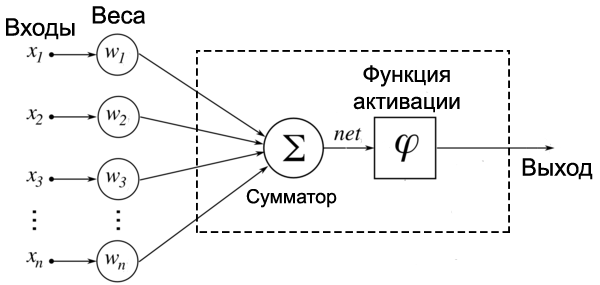
\includegraphics[width=0.7\linewidth]{img/perceptron.png}}
	\caption{Перцептрон}
\end{figure}

Упомянутые ученые также предложили способ объединения искусственных нейронов в сети, называемые нейронными сетями.
Нейроны, находящиеся на одном уровне обработки входных данных, объединялись в слои.
Слой, который принимает сигналы из внешнего мира, называется входным. Слой, который выдает сигналы во внешний мир, —
выходным. Остальные слои называются скрытыми \cite{sozykin}.

Рекуррентные нейронные сети -- подкласс нейронных сетей с обратными связями, которые
используют предыдущие состояния сети для вычисления текущего. Сеть строится из узлов, каждый
из которых соединѐн со всеми другими узлами. У каждого нейрона порог активации меняется со
временем и является вещественным числом \cite{bguir_rnn}. 
\begin{figure}[H]
	\center{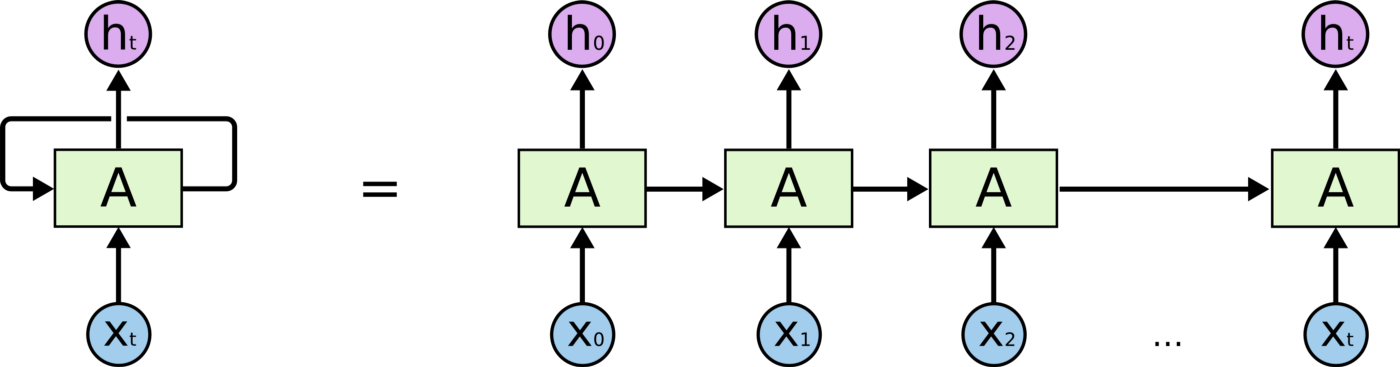
\includegraphics[width=0.7\linewidth]{img/rnn.png}}
	\caption{Иллюстрация работы рекуррентной нейронной сети}
\end{figure}

Автоэнкодерные сети -- подкласс нейронных сетей, для которых характерно наличие сжимающего слоя (энкодера) и восстанавлювающего словя (декодeра).
В процессе вычислений размерность входных данных данных понижается, над которыми далее могут производиться дополнительные преобразования, 
после чего размерность сжатых данных (латентного вектора) повышается \cite{vae}.
\begin{figure}[H]
	\center{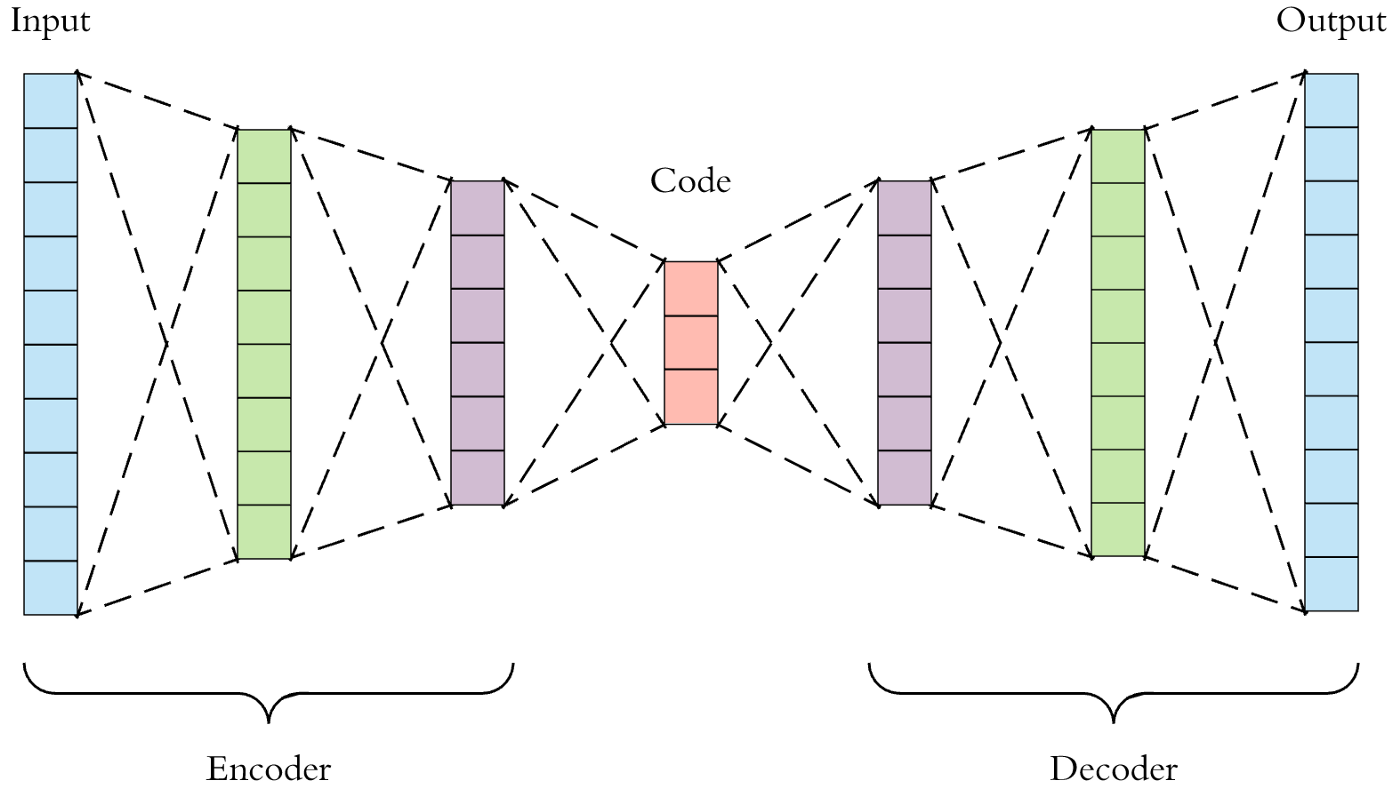
\includegraphics[width=0.7\linewidth]{img/autoencoder.png}}
	\caption{Иллюстрация работы автоэнкодера}
\end{figure}

Автоэнкодерные нейронные сети применяются для выделения наиболее важных информативных признаков 
(feature extraction) во входном пространстве образов, сжатия информации, очистки
данных от шумов, визуализации и классификации данных \cite{bgu_krasn}.

Самоорганизующиеся нейронные сети (self-organising neural networks)
характеризуются обучением без учителя, в результате которого проис-
ходит адаптация сети к решаемой задаче . Их разработал в 80-е гг. XX в.
финский ученый Т. Кохонен (T. Kohonen). Нейронные сети
Кохонена осуществляют топологическое упорядочивание входного
пространства образов, поступающих на сеть. Они широко применяются
в задачах распознавания и визуализации образов, оптимизации и
управления . В данной главе рассматривается архитектура, обучение и
функционирование самоорганизующихся нейронных сетей. Приводится алгоритм решения задачи коммивояжера с использованием сети Кохонена.

\chapter{Основные методы анализа аудиоданных. Анализ аудиоданных при помощи нейросетевых методов}
\chapter{Особенности подготовки аудиоданных}
\chapter{Кластеризация и классификация аудиоданных при помощи нейронных сетей}
\chapter{Сравнение полученных результатов с априорной классификацией}
\chapter{Общие результаты и выводы}